\documentclass[11pt,a4paper]{article}
\usepackage[utf8]{inputenc}
\usepackage[T1]{fontenc}
\usepackage[spanish,es-noshorthands]{babel}
\usepackage{amsmath,amssymb,amsthm}
\usepackage{bm}
\usepackage{geometry}
\geometry{margin=2.5cm}
\usepackage{graphicx}
\graphicspath{{../figuras/}}
\usepackage{float}
\usepackage{xcolor}
\usepackage{hyperref}
\hypersetup{colorlinks=true,linkcolor=blue!50!black,citecolor=blue!50!black,urlcolor=blue!50!black}
\usepackage{enumitem}
\usepackage{booktabs}
\newtheorem{definition}{Definición}
\newtheorem{remark}{Observación}
\newcommand{\R}{\mathbb{R}}
\newcommand{\thetavec}{\bm{\theta}}
\newcommand{\transp}{^{\top}}
\newcommand{\promptIA}[1]{\begin{center}\fcolorbox{gray}{gray!8}{\parbox{0.9\linewidth}{\small\textbf{[FIGURA -- PROMPT IA]}\\[2pt]#1}}\end{center}}
\title{\textbf{M4 --- Fundamentos de machine learning y optimización}\\[2pt]\large Puente al SciML: cómo se ajusta un modelo con datos}
\author{Proyecto Wilson--Cowan --- Iniciación a la I+D ITBA}
\date{\today}
\begin{document}
\maketitle
\tableofcontents
\bigskip

\noindent\textit{Requisito previo:} M1 (álgebra lineal y cálculo vectorial: gradiente, Jacobiano, Hessiano, autovalores, número de condición). Este documento es el \textbf{puente} entre esa base y los métodos de SciML que usamos para identificar los 10 parámetros de Wilson--Cowan (WC): la diferenciación automática de la Sección~\ref{sec:autograd} es la maquinaria que reaparece en M5 (residuo físico de la PINN) y en M6 (matriz de sensibilidad $J$ y análisis de Fisher). No es un curso de deep learning: es lo justo para leer y defender el pipeline de entrenamiento del proyecto.

\section{Aprendizaje supervisado, parámetros y función de pérdida}

\begin{definition}[Aprendizaje supervisado]
Tenemos pares de entrada--salida $\{(u_k,\,y_k^{\text{obs}})\}_{k=1}^{N}$ y un modelo $f_{\thetavec}$ con \textbf{parámetros} $\thetavec\in\R^{p}$. Aprender es buscar el $\thetavec$ que hace que las predicciones $\hat y_k = f_{\thetavec}(u_k)$ se parezcan lo más posible a los datos observados.
\end{definition}

\paragraph{Intuición.} Un modelo es una familia de funciones indexada por $\thetavec$; entrenar es elegir el miembro de esa familia que mejor explica los datos. La cercanía se mide con una \textbf{función de pérdida} (o costo) $L(\thetavec)$. La más común es el error cuadrático medio (MSE):
$$
L(\thetavec) \;=\; \frac{1}{N}\sum_{k=1}^{N}\big\lVert y_k^{\text{obs}} - f_{\thetavec}(u_k)\big\rVert^2 .
$$
Minimizar el MSE equivale a la estimación por máxima verosimilitud cuando el ruido de medición es gaussiano de varianza constante (este vínculo es exactamente el que conecta el MSE con la matriz de Fisher en M6).

\paragraph{Por qué en este proyecto.} Nuestro modelo NO es una red genérica: es \emph{gray-box}. La ``función'' $f_{\thetavec}$ es \textbf{integrar las EDOs de Wilson--Cowan} (ver M2) con un conjunto candidato de parámetros y comparar la trayectoria simulada $\hat y(t)=\hat E(t)-\hat I(t)$ con la observada $y^{\text{obs}}(t)$. Los ``parámetros'' son los 10 físicos de la Tabla canónica ($w_{EE},w_{EI},w_{IE},w_{II},\tau_e,\tau_i,a_e,a_i,\theta_e,\theta_i$), no pesos abstractos de una red. La pérdida es el MSE entre la salida medida $y=E-I$ y la simulada.

\begin{remark}
Los offsets $k_e,k_i$ \textbf{no} son parámetros libres: se derivan de las ganancias y umbrales para que el reposo $E=I=0$ sea equilibrio (ver M2/B3). Reducir el número de grados de libertad libres es una decisión de modelado que ayuda al condicionamiento del problema.
\end{remark}

\section{Descenso por gradiente, tasa de aprendizaje y mal condicionamiento}
\label{sec:gd}

\begin{definition}[Descenso por gradiente]
El gradiente $\nabla_{\thetavec} L$ apunta en la dirección de \emph{máximo aumento} de la pérdida. El descenso da pasos en la dirección opuesta:
$$
\thetavec_{t+1} \;=\; \thetavec_{t} \;-\; \eta\,\nabla_{\thetavec} L(\thetavec_{t}),
$$
donde $\eta>0$ es la \textbf{tasa de aprendizaje} (\emph{learning rate}).
\end{definition}

\paragraph{La tasa de aprendizaje.} Es la perilla más sensible. Si $\eta$ es muy chica, el entrenamiento se arrastra; si es muy grande, los pasos sobrepasan el mínimo y la pérdida diverge u oscila. No hay un valor universal: depende de la curvatura del paisaje $L(\thetavec)$.

\paragraph{Mal condicionamiento y zigzag.} El problema central aparece cuando el paisaje de la pérdida es un \textbf{valle largo y angosto}. Cerca de un mínimo, $L$ se aproxima por un paraboloide cuya forma la fija el Hessiano $H=\nabla^2 L$ (ver M1). Sus autovalores miden la curvatura en cada dirección propia; el \textbf{número de condición} $\kappa(H)=\lambda_{\max}/\lambda_{\min}$ mide cuán alargado es el valle. Cuando $\kappa$ es grande:
\begin{itemize}[nosep]
  \item una tasa $\eta$ que sea estable en la dirección \emph{muy curvada} (autovalor grande) es demasiado chica para avanzar en la dirección \emph{plana} (autovalor chico);
  \item el gradiente apunta casi perpendicular al eje largo del valle, así que el iterado \textbf{rebota de pared a pared} (zigzag) y progresa lentísimo hacia el mínimo (Figura~\ref{fig:valle}).
\end{itemize}
Esto no es un detalle académico: es \emph{el mismo} mal condicionamiento que en M6 diagnosticamos con Fisher+SVD como la razón por la que $w_{II}$ no se identifica. El valle plano de la optimización y el valle plano de la información de Fisher son la misma geometría vista desde el gradiente y desde la curvatura.

\begin{figure}[H]
\centering
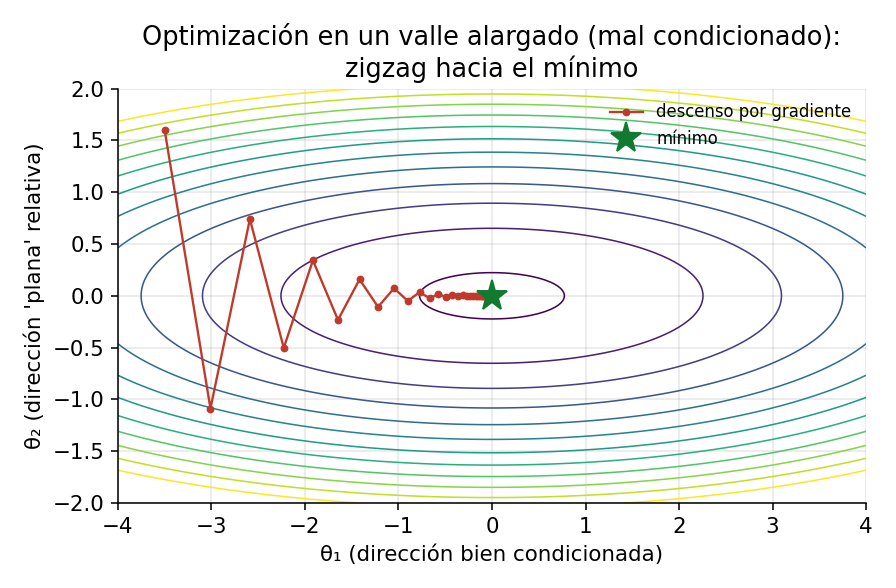
\includegraphics[width=0.75\linewidth]{fig_gradiente_valle.png}
\caption{Descenso por gradiente en un valle mal condicionado. La trayectoria zigzaguea entre las paredes empinadas mientras avanza a paso lento por el eje plano del valle. Aumentar $\eta$ para acelerar el eje plano hace divergir la dirección empinada. (figura del proyecto)}
\label{fig:valle}
\end{figure}

\section{Optimizadores del proyecto: Adam y L-BFGS}
\label{sec:opt}

El descenso por gradiente puro sufre el zigzag de la Sección~\ref{sec:gd}. Los optimizadores reales lo mitigan de dos formas complementarias, y el proyecto usa \textbf{las dos, en secuencia}.

\paragraph{Adam (primer orden, robusto).} Adam~\cite{kingma2015} usa solo el gradiente (primer orden) pero adapta el paso por coordenada: mantiene promedios móviles del gradiente (momento, que suaviza el zigzag) y de su cuadrado (para normalizar la escala de cada parámetro). Esto lo vuelve \textbf{robusto}: tolera gradientes ruidosos y mal escalados, y avanza bien aun sin ajustar $\eta$ con precisión quirúrgica. Su debilidad es que, cerca del óptimo, se estanca: da pasos pequeños y ruidosos sin converger fino.

\paragraph{L-BFGS (cuasi-Newton, refina al final).} L-BFGS~\cite{nocedal2006} es un método \textbf{cuasi-Newton}: aproxima la curvatura (el inverso del Hessiano) a partir del historial reciente de gradientes, sin formar ni invertir $H$ explícitamente (la ``L'' es de \emph{limited memory}). Al incorporar curvatura, \textbf{corrige el zigzag}: en un valle mal condicionado apunta hacia el fondo, no de pared a pared, y converge con precisión de muchas cifras cerca del óptimo. A cambio es más frágil lejos del mínimo (la aproximación de curvatura puede fallar con gradientes ruidosos) y más caro por paso.

\paragraph{Por qué se usan los dos.} La estrategia estándar en SciML, y la que seguimos, es una \textbf{cascada}:
\begin{enumerate}[nosep]
  \item \textbf{Adam para el grueso.} Arranca desde una inicialización cualquiera y lleva $\thetavec$ al entorno del óptimo de forma robusta, absorbiendo el ruido y el mal escalado inicial.
  \item \textbf{L-BFGS para afinar.} Toma el resultado de Adam como punto de partida (ya cerca del mínimo, donde su aproximación de curvatura es válida) y \textbf{refina} hasta el fondo del valle con alta precisión.
\end{enumerate}
Es la combinación de un ``martillo robusto'' seguido de un ``destornillador de precisión''. En la identificación de WC esto importa: el fondo del valle de $w_{II}$ es tan plano que Adam solo nunca lo asienta, y L-BFGS solo, arrancando lejos, se desestabiliza.

\section{Sobreajuste, validación y regularización L2}
\label{sec:overfit}

\begin{definition}[Sobreajuste]
Un modelo \textbf{sobreajusta} cuando reduce la pérdida sobre los datos de entrenamiento memorizando su ruido en lugar de capturar la estructura subyacente. Se detecta porque la pérdida de \emph{entrenamiento} baja pero la de \emph{validación} (datos no usados para ajustar) empieza a subir.
\end{definition}

\paragraph{Train / validación.} Partimos los datos en un conjunto de \textbf{entrenamiento} (se usa para mover $\thetavec$) y uno de \textbf{validación} (solo se mira para juzgar generalización). En el proyecto la validación es natural: entrenamos con ciertas trayectorias/estímulos y evaluamos sobre una trayectoria de \emph{test} distinta, típicamente un \emph{chirp} (ver \texttt{fit\_chirp\_test} en los resultados). Que el modelo identificado prediga bien un estímulo que no vio es la prueba de que recuperó la \emph{dinámica} y no un ajuste espurio.

\paragraph{Regularización L2 (mirada inicial).} Una forma clásica de frenar el sobreajuste y, sobre todo, de \textbf{domesticar el mal condicionamiento} es añadir a la pérdida una penalización cuadrática sobre los parámetros:
$$
L_{\text{reg}}(\thetavec) \;=\; \frac{1}{N}\sum_{k}\big\lVert y_k^{\text{obs}} - f_{\thetavec}(u_k)\big\rVert^2 \;+\; \lambda\,\lVert \thetavec - \thetavec_0\rVert^2 .
$$
El término $\lambda\lVert\thetavec-\thetavec_0\rVert^2$ tira de $\thetavec$ hacia un valor de referencia $\thetavec_0$ (un \emph{prior}), sumando información donde los datos no restringen. Geométricamente, agregar $\lambda I$ a la curvatura \textbf{rellena las direcciones planas} del valle y las vuelve estimables. El hiperparámetro $\lambda$ controla el balance sesgo--varianza: más $\lambda$ = menos varianza (estimación más estable) a costa de sesgo hacia $\thetavec_0$.

\begin{remark}
Dejamos aquí solo la intuición. El tratamiento completo --- Tikhonov/ridge, interpretación MAP bayesiana, la equivalencia $\lambda\to\infty$ con ``fijar'' un parámetro, y el barrido de $\lambda$ para $w_{II}$ (Exp A2, $\lambda^\star\approx 1.0$) --- va en \textbf{M6 (identificabilidad y OED)}, porque ahí la regularización aparece como remedio directo al valle plano de la matriz de Fisher.
\end{remark}

\section{Diferenciación automática (autograd)}
\label{sec:autograd}

Todo lo anterior necesita un ingrediente: el \textbf{gradiente} $\nabla_{\thetavec}L$ (y, en M6, el Jacobiano completo $J=\partial y/\partial\thetavec$). La \textbf{diferenciación automática} (AD, \emph{autograd}) los calcula de forma exacta y eficiente. Es la pieza técnica central de este documento porque es la base de M5 y M6.

\paragraph{Qué NO es.} Conviene despejar dos confusiones:
\begin{itemize}[nosep]
  \item \textbf{No es diferencias finitas.} No aproxima $\partial L/\partial\theta_j \approx (L(\theta_j+h)-L(\theta_j))/h$. Ese esquema es \emph{inexacto} (error de truncamiento y de redondeo peleando por $h$) y \emph{caro} (una evaluación del modelo por parámetro). AD da la derivada al nivel de precisión de máquina.
  \item \textbf{No es derivación simbólica.} No manipula fórmulas para producir una expresión cerrada de la derivada (que explotaría en tamaño). AD trabaja \emph{numéricamente}, propagando derivadas junto con los valores.
\end{itemize}
La idea: cualquier cómputo (incluso integrar una EDO paso a paso) es una composición de operaciones elementales; AD aplica la regla de la cadena a esa composición, acumulando derivadas operación por operación~\cite{baydin2018}.

\paragraph{Dos modos.} La regla de la cadena se puede recorrer en dos sentidos, y cuál conviene depende de la forma del problema (muchas entradas vs.\ muchas salidas):
\begin{itemize}[nosep]
  \item \textbf{Modo reverse (retropropagación).} Recorre el grafo hacia atrás desde la salida. Calcula el gradiente de \textbf{una} salida escalar respecto de \emph{todas} las entradas en (esencialmente) el costo de una evaluación del modelo. Es \textbf{barato cuando hay muchas entradas y una sola salida}: exactamente el caso de la pérdida $L$ (millones de parámetros posibles $\to$ un número). Es lo que usamos para $\nabla_{\thetavec}L$ al entrenar.
  \item \textbf{Modo forward (\texttt{jacfwd}).} Recorre el grafo hacia adelante, propagando la derivada respecto de una entrada a través de todo el cómputo. Da una \emph{columna} del Jacobiano por pasada, así que es \textbf{eficiente cuando \#parámetros $\le$ \#salidas}. Es el modo idóneo para construir la matriz de sensibilidad $J=\partial y/\partial\thetavec$: acá la ``salida'' es la trayectoria entera $y(t)$ (muchos puntos) y las ``entradas'' son solo 10 parámetros.
\end{itemize}

\paragraph{Por qué en este proyecto (la base de M5 y M6).}
\begin{itemize}[nosep]
  \item \textbf{M5 --- residuo físico (PINN).} La PINN penaliza que su predicción viole las EDOs de WC. Para armar ese residuo hay que derivar la salida de la red respecto del \emph{tiempo} (y de sus entradas); eso es AD. Sin diferencias finitas: el residuo físico se evalúa exacto.
  \item \textbf{M6 --- sensibilidad y Fisher.} La matriz $J=\partial y/\partial\thetavec$ se calcula por AD en \textbf{modo forward} (\texttt{jacfwd}), aprovechando que hay solo 10 parámetros contra una trayectoria larga. De $J$ salen la matriz de Fisher $J\transp J/\sigma^2$, su SVD y el diagnóstico de identificabilidad. Que $J$ sea \emph{exacta} (no una aproximación por diferencias finitas) es lo que hace confiable el análisis del cuello de botella $w_{II}$.
\end{itemize}
Además, entrenar el Neural ODE requiere \textbf{backpropagar a través del integrador}: como RK4 (ver M2) es una composición de operaciones diferenciables, AD atraviesa todos los pasos de integración sin que tengamos que escribir a mano ninguna derivada.

\section{Trucos de entrenamiento usados en el repo}
\label{sec:trucos}

Ajustar un Neural ODE \emph{gray-box} sobre un sistema oscilante y mal condicionado no funciona con un entrenamiento ingenuo. El repo usa tres trucos que vale la pena conocer:

\begin{itemize}[leftmargin=1.4em]
  \item \textbf{Warmup ``datos primero''.} En vez de castigar desde el arranque tanto el ajuste a datos como el residuo físico (o el término de dinámica), se \emph{empieza} priorizando el ajuste a los datos y recién después se sube el peso del término físico. Motivo: al principio los parámetros están lejos y el residuo físico produce gradientes enormes y engañosos; dejar que los datos lleven $\thetavec$ a una zona razonable primero estabiliza todo lo demás.
  \item \textbf{Congelar la red.} En un modelo con dos bloques --- la parte física con los 10 parámetros y la parte de red neuronal (features/corrección) --- conviene por etapas \textbf{congelar} (fijar, sin gradiente) uno mientras se ajusta el otro. Típicamente se fija la red para que los datos determinen primero los parámetros físicos, evitando que la red ``tape'' errores de los parámetros absorbiéndolos ella (lo que arruinaría la identificación).
  \item \textbf{Parada por meseta.} En vez de un número fijo de épocas, se monitorea la pérdida de validación y se \textbf{corta cuando deja de mejorar} (se amesetó) durante un número de épocas dado. Esto es \emph{early stopping}: previene el sobreajuste de la Sección~\ref{sec:overfit} y ahorra cómputo. Encaja con la cascada de la Sección~\ref{sec:opt}: se deja que Adam llegue a la meseta y ahí se pasa el control a L-BFGS para el afinado final.
\end{itemize}

\begin{remark}
Estos trucos son coherentes con toda la lógica del proyecto: el objetivo no es minimizar la pérdida a cualquier precio, sino \textbf{recuperar parámetros físicos identificables}. Por eso se cuida que sean los datos --- y no la flexibilidad de la red --- los que fijen $\thetavec$.
\end{remark}

\begin{thebibliography}{9}
\bibitem{goodfellow2016} I. Goodfellow, Y. Bengio y A. Courville, \textit{Deep Learning}, MIT Press, 2016.
\bibitem{nocedal2006} J. Nocedal y S. J. Wright, \textit{Numerical Optimization}, 2ª ed., Springer, 2006.
\bibitem{kingma2015} D. P. Kingma y J. Ba, ``Adam: A Method for Stochastic Optimization'', \textit{ICLR}, 2015.
\bibitem{baydin2018} A. G. Baydin, B. A. Pearlmutter, A. A. Radul y J. M. Siskind, ``Automatic differentiation in machine learning: a survey'', \textit{Journal of Machine Learning Research} 18(153):1--43, 2018.
\end{thebibliography}

\end{document}
